\documentclass{article}

\usepackage{ifthen}

\usepackage{kademliatrie}

\newcommand\subtrien[2]{
	\ifthenelse{\equal{#2}{0}}{
		{node \{#1\}}%
	}{
			node \{#1 \} \\
			child \{ \\
				\subtrien{#1 0}{\the\numexpr#2 -1\relax}
		\}
	}
}

\def\newnode{\node \{hi\};}

\begin{document}

%\countdown{}{3}
\subtrien{1}{0}

%\newtrie{1}

	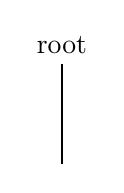
\begin{tikzpicture}[
		thick
	]
	
	\node{root}
	child {
		%{\subtrien{1}{0}}
		%\newnode
	};
	\end{tikzpicture}


\end{document}